\documentclass{beamer}
\usepackage[english]{babel}
\usepackage[justification=centering]{caption}
\usepackage{adjustbox}
\usepackage{booktabs}
\usepackage{multirow}
\usepackage{makecell}
\usepackage{array}
\usepackage[font=scriptsize]{caption}

\title{Comparing Structure Learning Algorithms Across Different Libraries}
\author{Tian Cheng Xia}
\institute{Alma Mater Studiorum $\cdot$ University of Bologna}
\date{06/02/2024}


\makeatletter
\definecolor{darkred}{rgb}{0.8,0,0}
\usetheme{default}
\usecolortheme{beaver}
\setbeamertemplate{navigation symbols}{}
\setbeamertemplate{footline}[frame number]
\setbeamercolor{caption name}{fg=darkred}
\setbeamercolor{description item}{fg=darkred}
\setbeamercolor{block title}{fg=darkred}
\setbeamertemplate{itemize item}{\color{darkred}$\blacktriangleright$}
\setbeamercolor{enumerate item}{fg=darkred}
\defbeamertemplate{description item}{align left}{\insertdescriptionitem\hfill}
\setbeamertemplate{title page}{
    \centering
    \vspace*{4em}
    {
        \usebeamercolor[fg]{title}\LARGE
        \inserttitle
    }

    \vspace*{1em}
    \small
    \insertauthor\\[0.5em]
    \insertdate\\
    
    \vspace*{3em}
    \small
    FAIKR Module 3\\
    \insertinstitute\\
}
\makeatother


\begin{document}


{
    \setbeamertemplate{footline}{}
    \begin{frame}
        \titlepage
    \end{frame}
    \addtocounter{framenumber}{-1}
}


\begin{frame}
    \frametitle{Aim}

    \begin{enumerate}
        \item Explore the available open-source Python libraries for Bayesian network structure learning.
        \item Compare the various structure learning algorithms implemented in them.
    \end{enumerate}
\end{frame}


\begin{frame}
    \frametitle{Libraries and algorithms}

    \begin{table}
        \scriptsize
        \centering
        \begin{tabular}{cccc}
            \toprule
            \multirow{2}{*}[-7pt]{\makecell{\textbf{Structure learning}\\\textbf{algorithms}}} & \multicolumn{3}{c}{\textbf{Library}} \\
            \cmidrule(r){2-4}
            & \makecell{\texttt{pgmpy}\\\texttt{bnlearn}} & \texttt{pomegranate} & \texttt{pyAgrum} \\
            \midrule
            \textbf{Score-based} &
                \makecell{
                    Hill-climbing\\
                    Exhaustive search
                } & 
                \makecell{A*} & 
                \makecell{
                    Hill-climbing\\
                    Tabu search\\
                    K2
                } \\
            \midrule
            \textbf{Tree-based} &
                \makecell{
                    Chow-Liu\\
                    Naive Bayes\\
                    Tree-augmented NB
                } &
                \makecell{Chow-Liu} & 
                \makecell{
                    Chow-Liu\\
                    Naive Bayes\\
                    Tree-augmented NB
                } \\
            \midrule
            \textbf{Constraint-based} &
                \makecell{PC} & 
                \makecell{---} & 
                \makecell{MIIC} \\
            \midrule
            \textbf{Hybrid} &
                \makecell{Max-min hill-climbing} &
                \makecell{---} & 
                \makecell{---} \\
            \bottomrule
        \end{tabular}
        \caption{Tested libraries and available structure learning algorithms.} 
    \end{table}
\end{frame}


\begin{frame}
    \frametitle{Evaluation approach}

    \begin{itemize}
        \item Evaluate on classification tasks.
        \item MLE as parameter learning algorithm.
        \item Variable elimination to solve queries.
    \end{itemize}
\end{frame}


\begin{frame}
    \frametitle{Datasets}

    \textbf{Apple quality}
    \begin{figure}
        \centering
        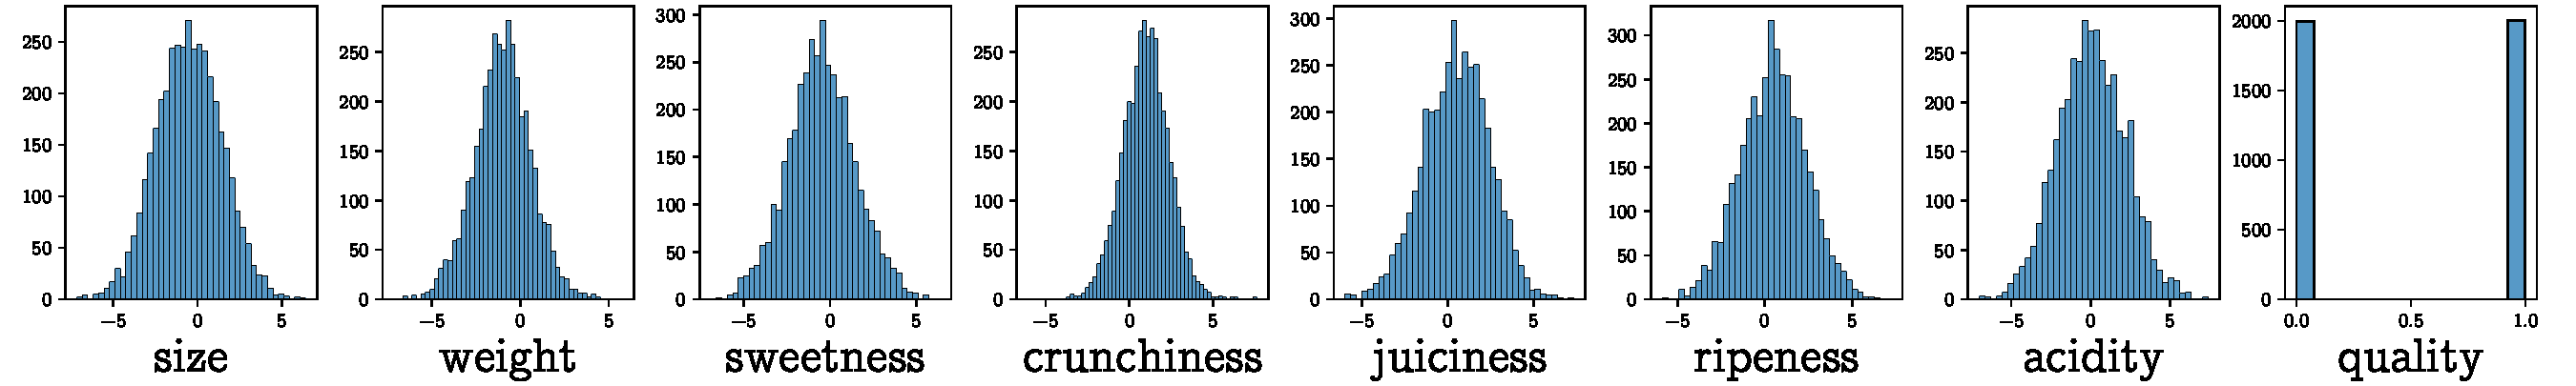
\includegraphics[width=\linewidth]{./img/apple_distribution.pdf}
        \caption{Apple quality data distribution}
    \end{figure}

    \textbf{Heart disease}
    \begin{figure}
        \centering
        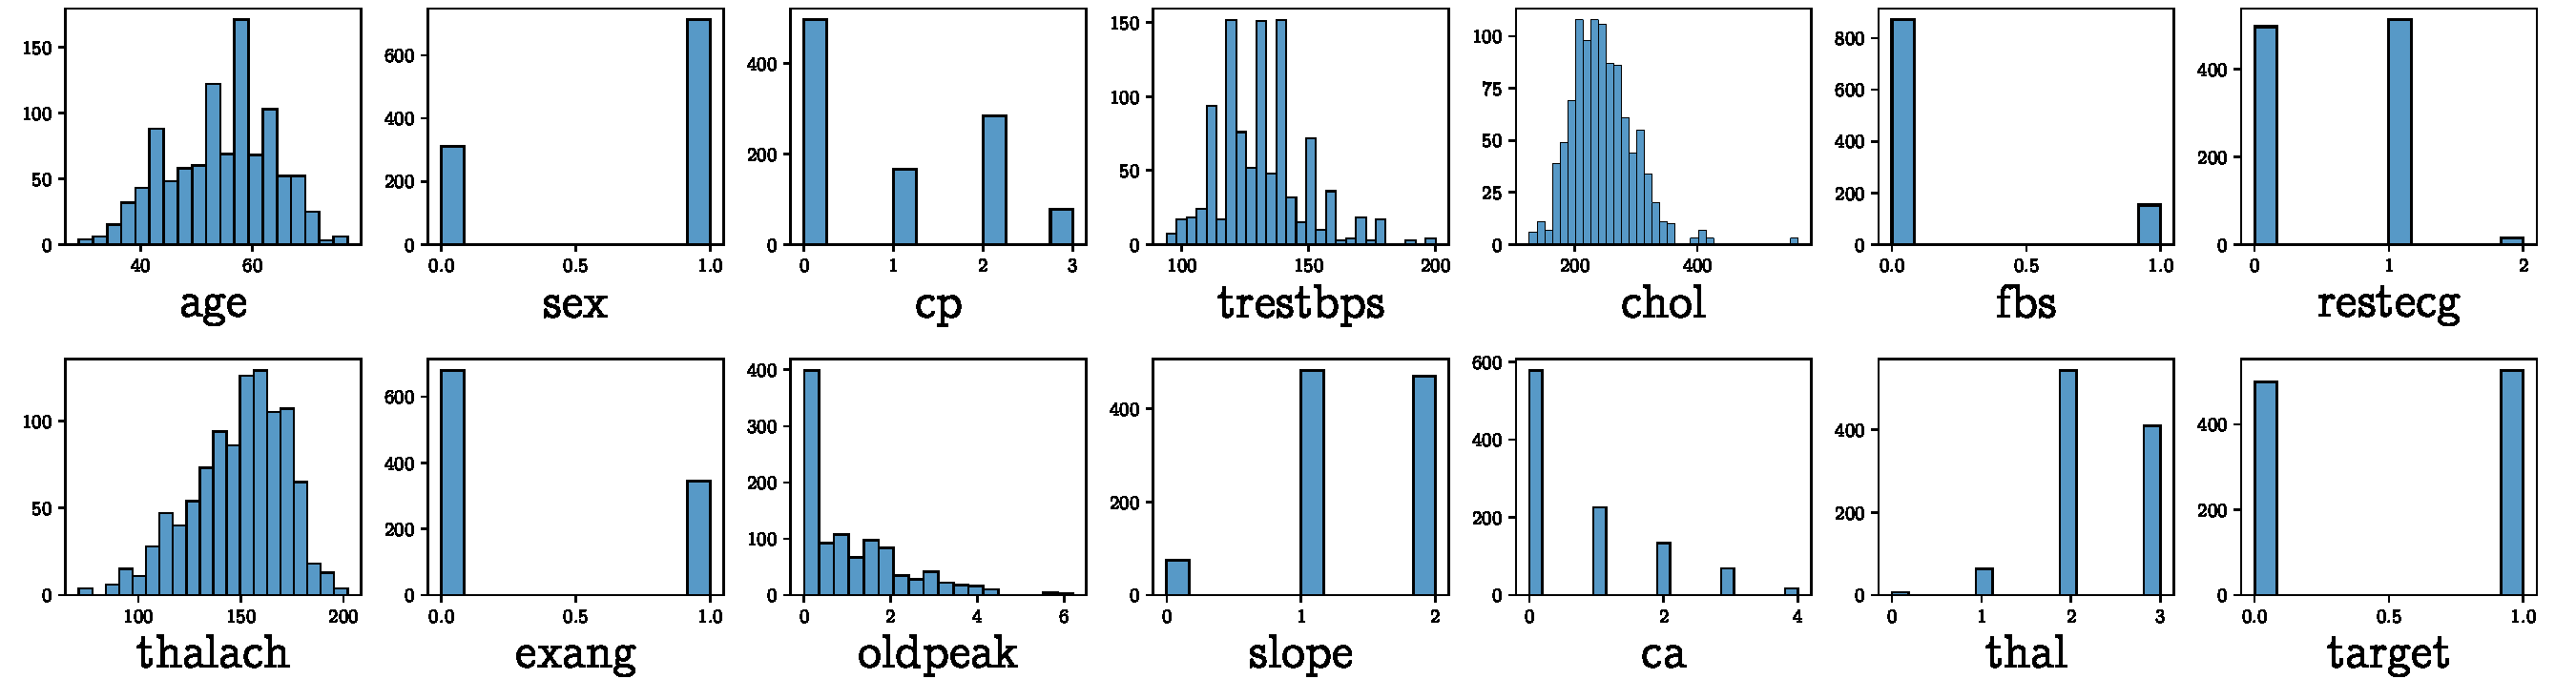
\includegraphics[width=\linewidth]{./img/heart_distribution.pdf}
        \caption{Heart disease data distribution}
    \end{figure}
\end{frame}


\begin{frame}
    \frametitle{Results}
    \framesubtitle{Accuracy vs number of edges}

    \begin{columns}
        \column{0.5\linewidth}
        \begin{center}
            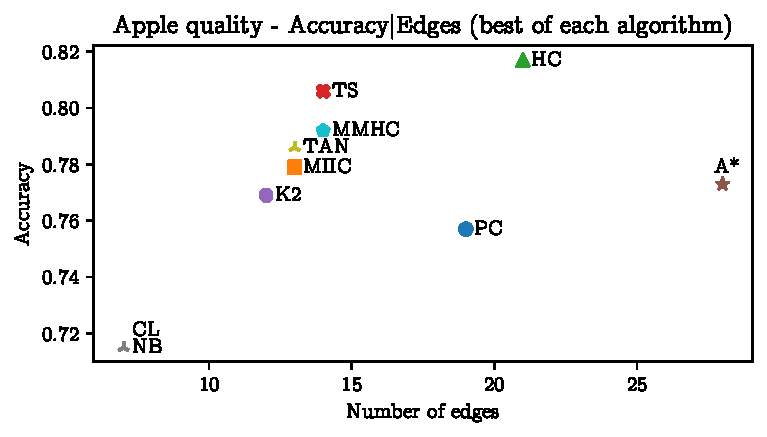
\includegraphics[width=\linewidth]{../report/img/apple_acc_edges.pdf}
        \end{center}

        \column{0.5\linewidth}
        \begin{center}
            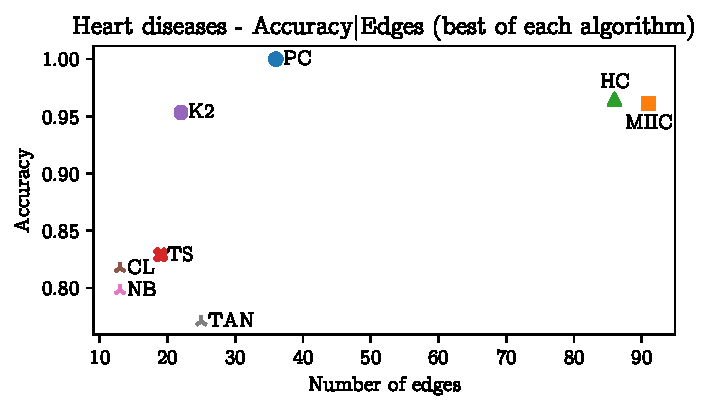
\includegraphics[width=\linewidth]{../report/img/heart_acc_edges.pdf}
        \end{center}
    \end{columns}

    \begin{itemize}
        \small
        \item Score-based methods work better on the apple quality dataset.
        \item Constraint-based methods work better on the heart disease dataset.
        \item Tree-based methods generally perform worse than the others but learn smaller topologies.
        \item The choice of the independence test/fitness score heavily influences the final result.
    \end{itemize}
\end{frame}

\begin{frame}
    \frametitle{Results}
    \framesubtitle{Accuracy vs CPU time}

    \begin{columns}
        \column{0.5\linewidth}
        \begin{center}
            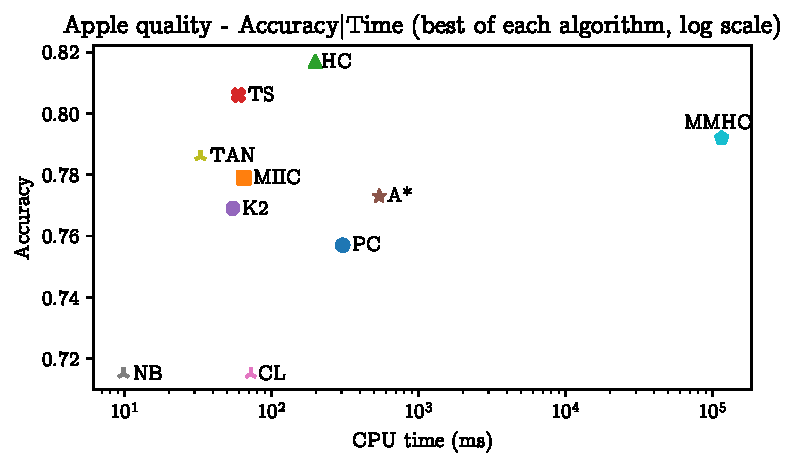
\includegraphics[width=\linewidth]{./img/apple_time.pdf}
        \end{center}

        \column{0.5\linewidth}
        \begin{center}
            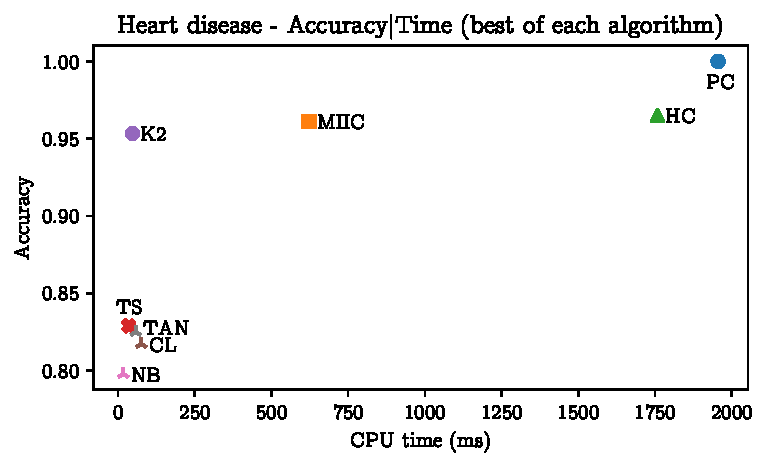
\includegraphics[width=\linewidth]{./img/heart_time.pdf}
        \end{center}
    \end{columns}

    \begin{itemize}
        \small
        \item Tree-based methods are generally the fastest.
        % \item The required learning time is dependent on the dataset.
        \item PC, hill-climbing, A*, and MMHC are among the slowest.
        \item Execution time and number of learned edges are not strictly related.
    \end{itemize}
\end{frame}


\begin{frame}
    \frametitle{Results}
    \framesubtitle{Visual comparison}

    \begin{figure}
        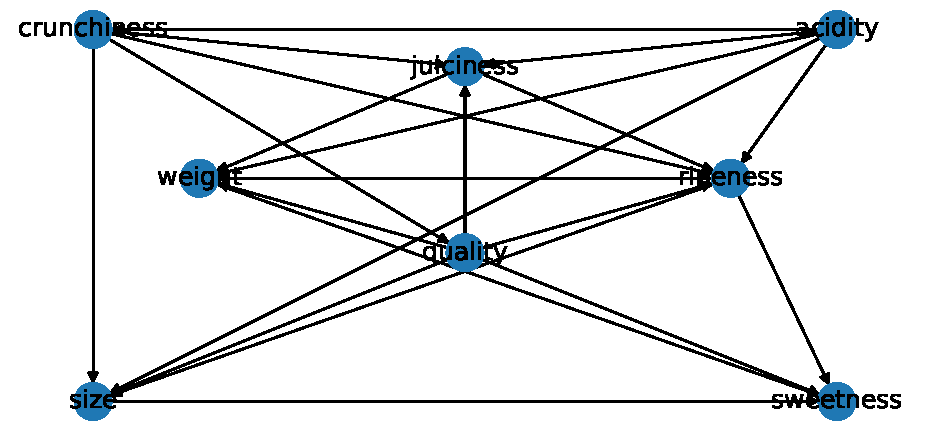
\includegraphics[width=0.6\linewidth]{./img/apple_hc.pdf}
        \caption{Apple quality -- Hill-climbing (K2 score) result}
    \end{figure}
    \begin{figure}
        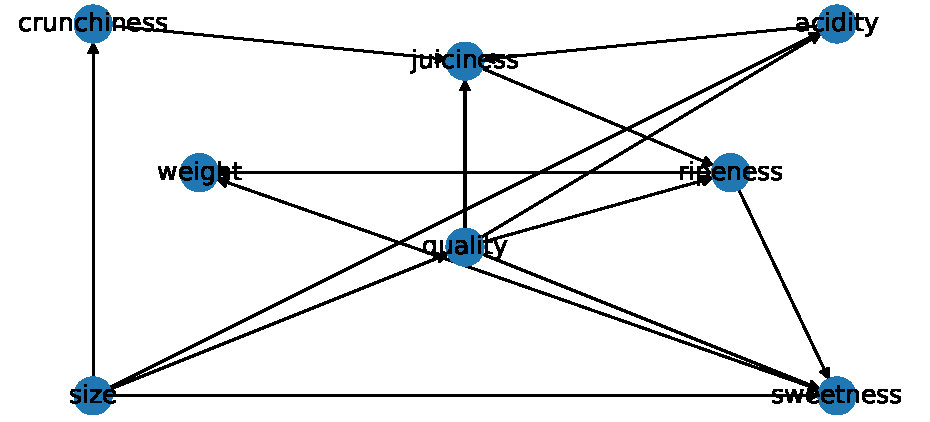
\includegraphics[width=0.6\linewidth]{./img/apple_ts.pdf}
        \caption{Apple quality -- Tabu search result}
    \end{figure}
\end{frame}


\begin{frame}
    \frametitle{Observations}

    \begin{itemize}
        \item Score-based and constraint-based methods generally perform better than tree-based methods.
        \item Tree-based methods generally produce simpler topologies.
        \item The choice of the best structure learning algorithm depends on the data.
    \end{itemize}
\end{frame}


\begin{frame}
    \frametitle{Limits}

    \begin{itemize}
        \item This mini-project only focuses on a classification-oriented evaluation.
        \item Only a small number of datasets have been experimented.
        \item The evaluation of the execution time is very informal and the different backends of each library must be taken into account.
    \end{itemize}
\end{frame}


\end{document}